\chapter{Android}\label{sec:Android}
This chapter will provide information about Android and Wear 2.0 technology. Why it was developed and what are the differences between previous version and other wear technologies.

\medskip

Android is a Linux based operating system for mobile and wear devices developed by Google. The main selling point of this system is that it's open-source project, meaning everyone can access the code and modify it as they wish. Android was mainly developed for mobile phones but in time moved beyond and at this time is implemented into all kinds of wear devices, tablets, televisions and even refrigerators or cameras \cite{WIGA}.

\section{Android system structure}\label{sec:AndroidSystemStructure}
Android is created as a stack, meaning there are functional modules stack on top of each other from Linux core over native libraries to applications as shown in \fref{fig6}. Android maintains complete software stacks to enable device creators to run and modify Android for their specific hardware. To support these modifications and testing every release has multiple "code lines" to separate stable versions from experimental work \cite{AOSP}.

\begin{figure}[H]
	\begin{centering}
		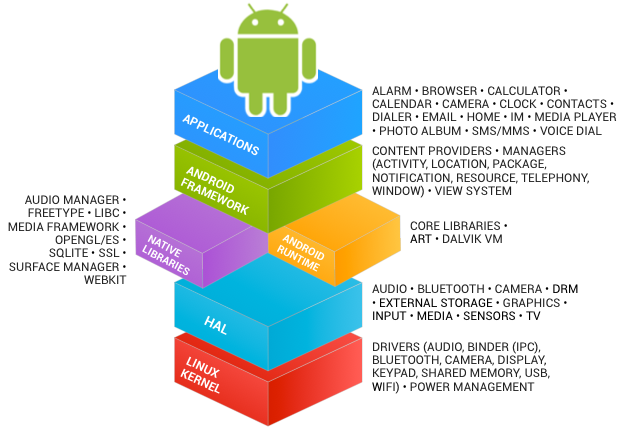
\includegraphics[width=0.6\textwidth]{img/android_stack}
		\par\end{centering}
	\caption{Android stack (source: \cite{AOSP})\label{fig:AndroidStack}}
	\label{fig6}
\end{figure}

There are multiple versions of Android system at this time and every single one has it's own version, code name and API level. Version codes are number identifications of a specific system version. Highest levels of these numbers are grouped into code names that are ordered alphabetically. As an example versions 8.0.0 and 8.1.0 have the same code name called Oreo. Finally API level is number identification for compatibility of specific application and it will be compared to API level of device Android system \cite{AOSP}\cite{AD}.

The highest part of the Android system stack are applications which extend device functionality and are written primarily in Java programming language \cite{SoASTaD}. These application are packaged into \verb|.apk| file, which is a zip archive, containing all application files like Java classes, layouts, images and more. Most important file is \verb|AndroidManifest.xml| that contains all meta-data about the application, such as permissions, package name, used components, versions and so forth. These application can be shared, for a nominal fee, via official market called Google Play. At the end of 2017 there were over three and a half million applications available in Google Play Store \cite{SoASTaD}\cite{NoAAiGPS}\cite{NoAA}.

Android is platform designed to be open source and free which makes it easy to create malicious applications. These application can bypass existing security and steal sensitive data, use telephony services or even gain control over the device \cite{ASIMPD}. Android has multiple ways to protect against such applications one of the most notable ones are Android Permission Framework and Google Play Protect \cite{SoASTaD}.

%T_ODO: describe Permissions and goofle play protect

\section{Wear technologies}\label{sec:WearTechnologies}
Interactive wearable, as an example smart watches, is a new part of mobile computers. Wear devices are categorically different from phones or tables in term of usage, design and user interfaces (UI). According to the app design guidelines by major vendors, users interact with wearable devices frequently throughout daily use. Each interaction is short, often less than 10 seconds, and is dedicated to simple tasks \cite{UtCoAWO}. 

Important thing to note is that there are multiple kinds of wear devices from smart watches, wristbands, cameras or even glasses \cite{MIWD}. Based on report from Gartner technology research, conducted in 2017, most used wear devices were Bluetooth headset, wristbands and smart watch \cite{GSWWDS}. Thanks to their small size wear devices are ideal to use for hands-free communication and health monitoring.

One problem with this diversity is hardware and software compatibility. Every device creator can create their own operating system for specific wear device and it can be difficult to develop custom applications for it. To avoid such problems this thesis is focused only on smart watch with Android Wear operating system. 

There are three main point to note with watch devices. First of all is small battery capacity that can be almost ten times smaller then in typical smart phone. The second point is display with around forty-times less pixels which completely changes properties. And final part is scaled down CPU with high efficiency \cite{UtCoAWO}. Last two points are main parts of lowering power consumption of smart watches but even with these cuts high-end watch devices can have really small battery life only in matter of few days or just hours.

\subsection{Android Wear}\label{sec:AndroidWear}
Android Wear is a version of Android OS tailored to small-screen wearable devices. There are not too many changes from system for smart phone but one of the main differences can be seen in UI since system had to be adjusted for watch size \cite{CSUITW}. Due to scaled down processing power of watches Android Wear wirelessly offloads data to the smart phone for heavy computing tasks, e.g., voice recognition \cite{UCAW}.

%Even thought this system got into top three wear systems it's first version was met with a lot of problems. Two types of wear apps

\section{Other wear technologies}\label{sec:OtherWearTechnologies}
Tizen, Pebble, Apple, Microsoft ...